\documentclass{article}
\usepackage{xcolor,mflogo}
\newcommand{\Rtxt}[1]{\textcolor{red}{#1}}
\newcommand{\TeXbook}{\textit{\TeX book}}
\newcommand{\TIP}{\textit{\TeX\ in Practice}}
\usepackage{X}
\usepackage{hyperref}
\hypersetup{%
xetex,
backref,
pdfpagemode=FullScreen,
bookmarksnumbered,
bookmarksopen,
colorlinks,
allbordercolors=1 1 1,
allcolors=blue,
pdfauthor={马起园},
pdfkeywords={TeX,基础知识,进阶},
pdftitle={TeX 一字一义}
}
\begin{document}
\title{\TeX 一字一义}
\author{马起园}
\maketitle
\newpage
{\sihao\hei 致\ 谢}

感谢丁叶,苏杰,冷轩,王侠兵,向伊梅,邓东升,周丽杏在本文写作过程中的不断指正。

把此文献给那些对我的啰嗦废话不厌烦的朋友们,顺便偿还欠下的笔头债。

\vskip 4ex
{\sihao\hei 支\ 持}

感谢{Fandol}基金会的强力打捞,以至本文不会石沉海底
\vskip 4ex
{\sihao\hei 技术后援}

马起园(\href{mailto:clerkma@gmail.com}{clerkma@gmail.com})

苏杰(\href{mailto:suxpert@gmail.com}{suxpert@gmail.com})

王侠兵(\href{mailto:wxiabing@gmail.com}{wxiabing@gmail.com})
\newpage
\tableofcontents
\newpage
\setcounter{page}{1}
\section{巵言}
这个材料是写给我的几个朋友看得,讲的是\TeX 的工作原理。这个材料也是我积累的结果,甚至为了弄清楚问题而去读我看不懂的《编译原理》(就是那本著名的\textit{Compilers},龙书,不过这本书还好理解,不过国内的书的话……还是算了,看国内编者的书总是培养不起来动手能力)。

要想深入理解\TeX 的工作细节,不是一件很简单的事情,我是看了很多材料才得到我现在笔下的东西的。现在在网上能找到很多关于\TeX 的材料,但是讲应用的偏多,讲原理,讲设计的几乎没有。我想我写的这点东西能够尽到绵薄之力吧。

我写这个材料的风格连我自己都感觉都很变态,我几乎是一边写一边改,甚至有些部分砍掉重写。但是请相信我写这个材料是不敢少说一句话的,宁肯多说几句话,虽然显得啰嗦废话。
\section{Token}
Token确实让我迷糊了一段时间,OED这本词典里的解释也曾经让我深度怀疑。另外查了数本英汉词典才心安了点儿,这个词在语言学中代表“语言符号”的意思,在相关的\TeX 文章中翻译成“标记”已经足够了。见如下引文(见\textit{OED}):
\begin{quotation}
f. \textsl{Semiotics}, etc. A particular and individual sign, as opposed to the type of which it is an instance.
\end{quotation}
其实纠结的不是英文涵义,而是中文翻译,这些词确实不好用另一种语言来表达,是一种翻译学上的通病。这个词在任何计算机语言中都会出现,我见过比较多的是在Lisp的教程中的例子 ,作为同时代的语言,这些术语内涵是一样的,现在这个词在一些讨论初级编程的书籍中好像用的少了,只在高级编程的话题(即编译原理)中有所提及,不过这个词的意思为什么来的还是值得去故纸堆里挖掘。在\TeX 的语境里中,这个词意思很容易理解,Knuth在\TeXbook(p.38)中写到:
\begin{quotation}
A token is either (a) \Rtxt{a single character} with an attached category code, or (b) \Rtxt{a control sequence}.
\end{quotation}
所以意思很明确:
\begin{itemize}
\item 带有\textit{category code}(类型码)的字符
\item 控制序列(\textit{Control Sequences})
\end{itemize}
这个引申出来两类标记:字符标记和控制标记。

更细致的划分是\TIP(Vol.III, pp.4-5)给出的:
\begin{itemize}
\item 字符标记(\textit{Charcater tokens})
\item 控制标记(\textit{Control sequence tokens})
\begin{itemize}
\item 控制词(\textit{Control words}),如\verb!\hskip!
\item 控制符(\textit{Control symbols}),如\verb!\&!
\end{itemize}
\item \Rtxt{变量标记}(\textit{Parameter tokens}),从\verb!#1!到\verb!#9!
\end{itemize}
值得注意的是空格在控制标记中依照不同的类别起不同的作用:在控制词后会被忽略,形象一些的说法是“被吃掉”;在控制符后是起作用的,例如最大名鼎鼎的“\verb*!\ !”这个强制输出空格的命令,但是当存在一个空格时,多余的也会“被吃掉”,如“\verb*!\   !”只会生成一个空格,其余不起作用。

在使用\TeX{}过程中,输出空格有三种方式:
\begin{enumerate}
\item 使用空组,\verb!{}!
\item 使用\verb!\space!
\item 使用\verb*!\ !
\end{enumerate}

\TIP 给出的变量标记是在\TeXbook 中被忽略的一个小概念。另外对于字符标记,在某些控制标记后面,多个字符标记会形成关键字,如
\begin{verbatim}
\font\Aug\augie.ttf at 10pt
\end{verbatim}
at便是关键字。

掌握Token的基本的概念,对整个\TeX 的理解都会有很大帮助,Knuth给出了下列注释\TeXbook(p.38):
\begin{quotation}
It is important to understand the idea of token lists, if you want to gain \Rtxt{a thorough understanding of \TeX}, and it is convenient to learn the concept by thinking of \TeX{} as if it were a living organism.
\end{quotation}

回到原点,\TeX 怎么说都是一种编程语言,只不过产出的事物不一样,C语言能创造出有生产力的可执行文件,而\TeX 生成的是文档。所以理解\TeX 的开始不能不严谨,一定要把它和我们通常认为上的编程语言等量齐观才行。关于\TeX 中的标记,后面还会提到,这里仅介绍这一部分。另外关于C语言中的标记,有必要让读者进一步阅读,最好的一本书是Peter Prinz和Tony Crawford合著的\textit{C in a Nutshell}的“第1章 C编译器运行原理”。
\section{Category Code}
上面提到了带category code的字符标记,这个词的翻译已经给出来了,如上“类型码”。这个类型码主要是用来标记字符属性的,来辨别字符在\TeX 中的作用的。下面是plain \TeX 定义的和类型码对应代一些专有用途的字符(\TIP, Vol.III, p.6),共17种:

\begin{table}[!ht]
\begin{center}
\begin{tabular}{llllll}
0&转义符&\verb!\!&1&组开始&\verb!{!\\
2&组结束&\verb!}!&3&数学转换&\verb!$!\\
4&对齐&\verb!&!&5&行结束&\verb!<return>!\\
6&变量&\verb!#!&7&上标&\verb!^!\\
8&下标&\verb!_!&9&忽略字&\verb!<null>!\\
10&空格&\verb*! !或\verb!tab!&11&字母&\verb!A-Z!和\verb!a-z!,有时为\verb!@!\\
12&其他字符&\verb!0-9!和其他未在列字符&13&激活符&\verb!~!\\
14&注释符&\verb!%!&15&不可用字符&\verb!<delete>!\\
\Rtxt{16}&控制序列&&&\\
\end{tabular}
\end{center}
\end{table}

上面的16不是很常用(而且也是\TIP 加的),只有在\verb!\ifcat!及一些类似结构中需要使用。定义字符的类形码要用到如下:\newline
\verb!\catcode!\verb!<character>=<category code>!\newline
示例如下:\newline
\verb!\catcode!\verb!'173=1!\newline
\verb!\catcode!\verb!`\{=1!

这些类型码,对应\TeX 来说,是一个来区别排版元素和非排版元素的东西,至于怎么分析?后文会提及。
\subsection{\textsc{INI}\TeX 初步}
\textsc{ini}\TeX 初始化时,差不多所有的字符的类型码是12,但是有下列意外:
\begin{enumerate}
\item \verb!\!为0
\item \verb*! !为5
\item \verb!<null>!为9
\item \verb!<return>!为10
\item \verb!a-z, A-Z!为11
\item \verb!%!为14
\item \verb!<delete>!为15
\end{enumerate}
\section{编码,字符}
\subsection{编码}
\begin{enumerate}
\item \verb!ASCII!
\item \verb!EBDIC!
\item \verb!KOI8-R, KIO8-U, KOI7!
\item \verb!BIG5!
\item \verb!GBK, GB-2312, GB-18030!
\item \verb!JIS, ISO/IEC 2022, Shift JIS, EUC!
\item \verb!UNICODE!
\end{enumerate}
\subsection{字符}
\section{\TeX 的工作流程}
这里解释一下为什么“标记”和“类型码”是很重要且基础的命令。那么我们来看一下\TeX 对原文件的处理方式(基本上是从\textit{\TeXbook}中的形象解说写过来的,这个说法已经是经典了,此处解说引用\textit{The Advanced \TeXbook} pp.19-20,在\textit{\TeX{} by Topic}中将这个处理阶段分成了四个,不过和我这个分类差别不大,而且给出来了详细的解释,所以下面的文本是综合两本书的结果)。先给出一句引言:
\begin{quotation}
It is convenient to learn the concept (of tokens) by thinking of \TeX{} as if it were \Rtxt{a living organism}.
\end{quotation}
\begin{enumerate}
\item 源文阶段。即未处理的文本,在计算机看来是数据
\item 读取阶段,这时候涉及的命令是\verb!\input!,经过读取后,源文就从一堆1和0变为了某种编码下的字符
\item 咀嚼阶段,\TeX 将读取的字符翻译为标记,这个过程中\TeX 要一个减法和加法,减法是把某些多余的空格删除,加法是在空行结尾处加\verb!\par!,至于带有\verb!\!的,\TeX 将会读取其后的字符来组成一个单独的标记,这一阶段几乎就是\TeX 在源文编码和类型码之间的翻译,\TeX 中的类型码相当于\TeX 将源文字符编码翻译成\TeX 能读懂的语言要对应的一个词典,不过和一般翻译的不同的就是这个词典太精悍了。实际上还存在着一种字符之间的转换,比如\verb!^^+!被替换为^^+,这是因为某些因为终端或者编辑器甚至操作系统的原因而不能直接输入该字符,所以要用这种转换(具体的转换是两个字符之间相差64,上例中+和k的ASCII编码分别是43和107,使用\verb!^^+!和\verb!^^k!分别获得^^+和^^k)。在咀嚼阶段,就是这两种处理
\item 吞咽阶段,展开标记(凡是能展开的标记即为“宏”)和某些命令,不能展开的便不展开。这个阶段比较特殊的几个有\verb!\expandafter!,\verb!\noexpand!,\verb!\the!三个命令,括号也会经过特殊处理
\item 消化阶段,执行上一阶段带来的标记流(\textit{tokens stream})这些标记主要用来构成列(\textit{list}: 大文本单位)和模式识别
\end{enumerate}

在\TIP (Vol.3 p.1)中给出了更抽象的说法是:\textit{lexical analyzer}(语法分析器,咀嚼阶段),\textit{parser}(剖析器,吞咽阶段)和\textit{code generator}(代码发生器,消化阶段)。有一个更形象的图,见下面图\ref{fig1}。
\begin{figure}[!ht]
\centering
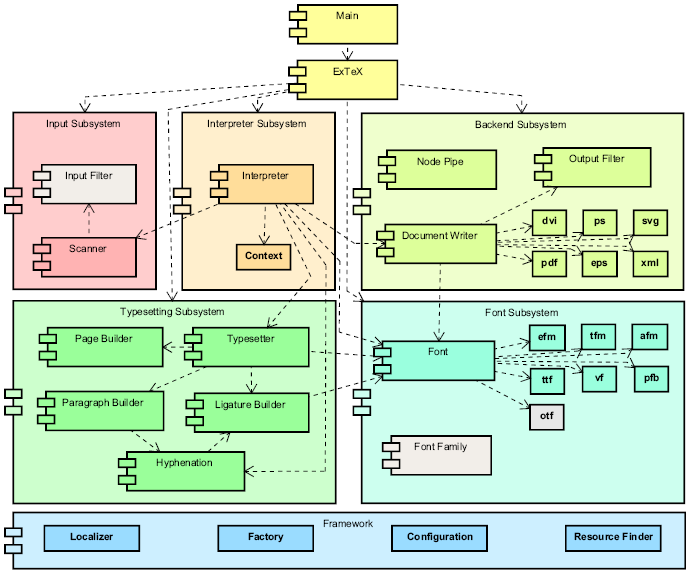
\includegraphics[width=.6\textwidth]{components.png}
\caption{\TeX 工作原理示意图($\epsilon\chi$\TeX 为例,显然这个图要比我们这里谈到的要多很多,能掌握这个图了就能理解\TeX 的精髓了)\label{fig1}}
\end{figure}

\section{Registers一般}
寄存器在\TeX 中是连接程序和排版版面的的一个概念,它实际上是\TeX 运行时所用到的一小块内存,这个概念所表达的直接的意思是一些排版元素的集合。掌握寄存器这个概念应该把它和其他语言中的变量类型联系起来,二者比较相似。下面的每一类别的寄存器都有256个寄存器。
\begin{enumerate}
\item 计数器寄存器(\textit{Counter} Registers),\verb!\count!类,默认为\texttt{0}
\item 长度寄存器(\textit{Dimension} Registers),\verb!\dimen!类,默认为\verb!0pt!
\item 胶寄存器(\textit{Glue} Registers),\verb!\skip!类,默认为\verb!0pt plus 0pt minus 0pt!
\item 数学胶寄存器(\textit{Math Glue} Registers),\verb!\muskip!类,默认为\verb!0mu plus 0mu minus 0mu!
\item 标记寄存器(\textit{Token} Registers),\verb!\toks!类,默认为空
\item 盒子寄存器(\textit{Box} Registers),\verb!\box!类,默认为\texttt{void}
\end{enumerate}
这个分类表明的是这些元素的类别。在\TeX 输出格式上就是这些寄存器的大量运用,包括组合,或者单独使用,\TeXbook 中的附录D所谓的Dirty Tricks属于高阶的使用,或者用现代的话来说是Hacking。

使用寄存器,要经历下面五个过程(见\textit{The Advanced \TeXbook},p.16):
\begin{enumerate}
\item {\hei 分配} 通过\verb!\new!\textit{xx}和\verb!\def!\textit{xx}命令完成
\item {\hei 赋值} 抹除寄存器旧值
\item {\hei 应用} 寄存器可以使用数次,但是盒子寄存器例外
\item {\hei 外显} 写入文档和\texttt{.log}文件,这个命令对于盒子寄存器来讲会很有用
\item {\hei 写入} 将寄存器值写入文件,但是盒子寄存器依然例外
\end{enumerate}

还有{\hei 保留寄存器}。寄存器分配。
\section{寄存器详解}
这里用很长的篇幅来解释\TeX 中的各种寄存器。
\subsection{长度}
长度在以前已经介绍过两种,其实有三种:
\begin{enumerate}
\item 绝对长度
\item 相对长度,依赖与字体
\item 无限长度
\end{enumerate}
\subsubsection{\TeX 中的绝对长度}
\begin{itemize}
\item \rule{1in}{1pt},\verb!1in!
\item \rule{1cm}{1pt},\verb!1cm!
\item \rule{1mm}{1pt},\verb!1mm!
\item \rule{1pc}{1pt},\verb!1pc!
\item \rule{1bp}{1pt},\verb!1bp!
\item \rule{1pt}{1pt},\verb!1pt!
\item \rule{1dd}{1pt},\verb!1dd!
\item \rule{1cc}{1pt},\verb!1cc!
\item \rule{1sp}{1pt},\verb!1sp!
\end{itemize}

\TeX 支持的长度都在这里了,已经眼花缭乱了吧?\TeX 中有这么多单位主要是支持不同国家的度量衡,虽然中国的传统度量衡“丈”“尺”“寸”没有包含在内。而另外一个原因是基于排版质量考虑的,因为好的排版系统是能够处理多国长度单位的。这里面的\verb!sp!比较特殊,它是\TeX 中的标准长度,或者说,除此之外的单位都要转换成\verb!sp!,这个词的翻译可以是“测点”。还有一点需要提出来的是这些长度都可以是小数,比如可以是\verb!2.37pt!,还有就是支持不同的计数形式,即\verb!2,37pt!也是支持的。

这些长度用来干什么?计算机不会用尺子边量边思考,只会算。所以这些长度能让\TeX 知道生成的版面是什么样的,还有就是另一些元素,比如盒子是有长度的属性的。

\TeX 中支持的长度最大为$(2^{31}-1)$\verb!sp!。

\verb!in!来源于\textit{inch},完全是英制单位。12个英寸就是一英尺。但是我觉得英制单位在换算上,够麻烦的,倒是和中国的旧制有一拼。如果不是要用到英国的排版技术材料,不建议使用\verb!in!来做长度单位。

\verb!pt!是\textit{point}的缩写,国内翻译成“点”或“磅”。这也是国内使用最为广泛的长度单位,主要用来确定字号。另一个中国用到比较多的是“级”。这个是根据机械齿轮来算出来的一个单位,现在的电子排版时代,意义已经不大。顺便介绍一下汉字的字号这个可以归类到相对长度定义的概念(这里给出最早的七级字号,注意表的内容,1858):
\begin{table}[!ht]
\begin{center}
\begin{tabular}{llllllll}
\hline
字号&一&二&三&四&五&六&七\\
\hline
汉名&显&明&中&行&解&注&珍\\
\hline
\end{tabular}
\end{center}
\end{table}
现在用的字号体系就是根据这个来的,不过根据实际情况有过增订,不过略显遗憾的是,现在不同的排版软件的汉字字号都不是一致的。

\verb!cm!和\verb!mm!就不用怎么细说了,国际单位制的衍生单位,它的通用性和阿拉伯数字一样,早就跨国界统一使用了。

\verb!pc!是另一个系统的长度单位,来源于英语的\textit{pica},下面是一些关于这个长度系统的一些东西:
\begin{table}[!ht]
\begin{center}
\begin{tabular}{ccccc}
\hline
\textit{pica}&\textit{small pica}&\textit{two-line pica}&\textit{double pica}&\textit{canon}\\
\hline
$\frac{1}{6}in=12pt=11.33dd$&$11pt$&$24pt$&$22pt$&$48pt$\\
\hline
\end{tabular}
\end{center}
\end{table}
这个是我最头疼的一个单位制,甚至碰到了\textit{English}这个长度单位(对,这个确实是个单位,不要怀疑,因为这个,但是我不解释,我快崩溃了)。

该讲\verb!cc!这个单位了,它是以古罗马著名演说家\textit{Cicéro}的名字命名的,主要用在德法两国,有个形象的说法是,“德法版的\textit{pica}”,而且据信是根据西塞罗的书信初版印刷字体的大小沿用下来的,不过这个名字是否出自德法国人之手,尚不可知。

还有哪个没讲到?\verb!pt!,\verb!bp!和\verb!dd!。为什么放在一起讲?因为它们是都是点制。我们拿这些点制换算到\verb!in!或\verb!pt!:
\begin{center}
$72.27pt=1in$, $72bp=1in$, $1157dd=1238pt(0.93dd=1pt)$
\end{center}

我们看见这三种点制的差别在哪里了吧?\verb!dd!有个称谓是“欧洲点制”。而\verb!bp!是PostScript语言中的单位,但是在PostScript语言中也是被称为\verb!pt!,这一点要注意。
\subsubsection{相对长度}
\begin{enumerate}
\item \verb!em!
\item \verb!en!
\item \verb!mu!
\end{enumerate}
\subsubsection{无限长度}
\begin{enumerate}
\item \verb!fil!
\item \verb!fill!
\item \verb!filll!
\end{enumerate}
\subsubsection{长度寄存器}
有256个寄存器,使用长度寄存器如下:
\begin{enumerate}
\item \verb!\dimendef\adimen=2!
\item \verb!\newdimen\xdimen!
\end{enumerate}
使用时要注意:
\begin{enumerate}
\item 长度寄存器可直接赋值,如\verb!\adimen=12pt!
\item 长度寄存器值可以传递,如\verb!\xdimen=.3\adimen!
\item 可使用负值 
\end{enumerate}
盒子使用\verb!\ht!,\verb!\wd!\verb!\dp!来分别获取其高度,宽度和深度。
\subsubsection{长度变量}
\begin{enumerate}
\item \verb!\hfuzz, \vfuzz, \overfullrule!
\item \verb!\prevdepth, \lineskiplimit!
\item \verb!\maxdepth, \splitmaxdepth, \boxmaxdepth!
\item \verb!\delimitershortfall, \nulldelimiterspace, \scriptspace, \mathsurround, \predisplaysize, \displaywidth, \displayindent!
\item \verb!\parindent, \hangindent!
\item \verb!\hoffset, \voffset!
\end{enumerate}
\subsection{胶}
有256个胶,使用胶寄存器如下:
\begin{enumerate}
\item \verb!\skipdef\askip=2!
\item \verb!\newskip\xskip!
\item \verb!\muskipdef\ma=2!
\item \verb!\newmskip\mx!
\end{enumerate}
胶的赋值和长度寄存器的赋值一样。但是数学胶不能和\verb!\hskip!和\verb!\vskip!一起使用。

\subsubsection{胶变量}
\begin{enumerate}
\item \verb!\baselineskip, \lineskip!
\item \verb!\topskip, \splittopskip!
\item \verb!\parskip, \leftskip, \rightskip, \emergencystretch!
\item \verb!\abovedisplayskip, \abovedisplayshortskip, \belowdisplayskip, \belowdisplayshortskip!
\end{enumerate}

\subsection{盒子}
0-9编号盒子保留使用,无盒子变量。定义新盒子要使用\verb!\newbox\abox!,且从10开始计数。在使用时利用\verb!\copy, \box!等来排印盒子内的内容。

寄存器有三种状态:
\begin{enumerate}
\item 水平
\item 垂直
\item 空
\end{enumerate}
\subsubsection{盒子取还}
把盒子寄存器编号和\verb!\abox!等看作index:
\begin{enumerate}
\item \verb!\box<index>!
\item \verb!\copy<index>!
\item \verb!\unhbox<index>!
\item \verb!\unhcopy<index>!
\end{enumerate}

\subsection{垂直盒子}
\section{排版算法基础}
\TeX 是图灵完备的,也就是说,它可以看作一种图灵机的实现。在实现上,\TeX 是人为营造的图灵完备体系。
\subsection{运算}
\begin{enumerate}
\item 加法和减法,下面的\verb!by!是关键字
\begin{verbatim}
\advance<integer variable> by <number>
\advance<dimen variable> by <dimen>
\advance<glue variable> by <glue>
\advance<muglue variable> by <muglue>
\end{verbatim}
\item 乘法
\begin{verbatim}
\multiply<numeric variable> by <number>
\end{verbatim}
\item 除法
\begin{verbatim}
\divide<numeric variable> by <number>
\end{verbatim}
\end{enumerate}
\subsection{判断}
\begin{enumerate}
\item \verb!\if<token1><token2>!,判断两个标记是否一样
\item \verb!\ifcase<number>!,条件选择,要配合\verb!\or!使用
\item \verb!\ifcat<token1><token2>!,在\TeXbook 中使用稀少
\item \verb!\ifdim<dimen1><relation><dimen2>!
\item \verb!\ifeof<4-bit number>!
\item \verb!\iffalse!
\item \verb!\ifhbox<8-bit number>!
\item \verb!\ifhmode!
\item \verb!\ifinner!
\item \verb!\ifmmode!
\item \verb!\ifnum<number1><relation><number2>!
\item \verb!\ifodd<number>!
\item \verb!\iftrue!
\item \verb!\ifvbox<8-bit number>!
\item \verb!\ifvmode!
\item \verb!\ifvoid<8-bit number>!
\item \verb!\ifx<token1><token2>!
\item \verb!\fi!
\item \verb!\else!
\item \verb!\or!
\end{enumerate}
\subsection{循环}
\verb!\loop\repeat!这个循环结构是plain \TeX 扩展出来的,实际上它们的定义是
\begin{verbatim}
\def\loop#1\repeat{\def\body{#1}\iterate}
    \def\iterate{\body \let\next=\iterate
    \else \let\next=\relax\fi \next}
\end{verbatim}
\section{宏语言和宏}
\TeX 是一种著名的宏语言,Lisp名家Paul Graham在他的两本Lisp书籍中都提到了\TeX ,并指出了作为宏语言的\TeX 的一个重要特征:自下而上。所谓的“自下而上”的含义就是,这种语言具有扩展性,能够用来设计高一层次的语言,对所设计的程序量体设计语言。另外一位UNIX界标杆人物Eric Steven Raymond则批评\TeX 语言写出来的东西太难阅读了。但事实是,只要有宏,任何一种语言或许都会最终变得很难阅读,关键在于宏的使用者的使用程度。

对初学者的一个忠告是:一定要把\TeX 当作一门语言来学,可以想象成是\verb!C!,\verb!Lua!等语言。而且还要树立另外一个观念:\TeX 不可速成。西方的谚语:
\begin{center}
Roman was not build in \Rtxt{a} day.
\end{center}

我们常见如下名词:宏,命令,基本控制序列和宏包。这四个类似的概念在英文中不会引起混乱,但是汉语中,由于使用的语境不同,某些人对着这几个概念会产生误解。

请读者先试验如下代码(这是著名的xii.tex):
\begin{verbatim}
 \let~\catcode~`76~`A13~`F1~`j00~`P2jdefA71F~`7113jdefPALLF
 PA''FwPA;;FPAZZFLaLPA//71F71iPAHHFLPAzzFenPASSFthP;A$$FevP
 A@@FfPARR717273F737271P;ADDFRgniPAWW71FPATTFvePA**FstRsamP
 AGGFRruoPAqq71.72.F717271PAYY7172F727171PA??Fi*LmPA&&71jfi
 Fjfi71PAVVFjbigskipRPWGAUU71727374 75,76Fjpar71727375Djifx
 :76jelse&U76jfiPLAKK7172F71l7271PAXX71FVLnOSeL71SLRyadR@oL
 RrhC?yLRurtKFeLPFovPgaTLtReRomL;PABB71 72,73:Fjif.73.jelse
 B73:jfiXF71PU71 72,73:PWs;AMM71F71diPAJJFRdriPAQQFRsreLPAI
 I71Fo71dPA!!FRgiePBt'el@ lTLqdrYmu.Q.,Ke;vz vzLqpip.Q.,tz;
 ;Lql.IrsZ.eap,qn.i. i.eLlMaesLdRcna,;!;h htLqm.MRasZ.ilk,%
 s$;z zLqs'.ansZ.Ymi,/sx ;LYegseZRyal,@i;@ TLRlogdLrDsW,@;G
 LcYlaDLbJsW,SWXJW ree @rzchLhzsW,;WERcesInW qt.'oL.Rtrul;e
 doTsW,Wk;Rri@stW aHAHHFndZPpqar.tridgeLinZpe.LtYer.W,:jbye
\end{verbatim}
这个例子很极端,但是也侧面说明,\TeX 也可以用来写出生涩难读的代码。
\subsection{宏}
宏是英语Macro的翻译,可以简单理解为文本的替换,但是实际上要比这个复杂得多,Knuth的\TeXbook(p.199):
\begin{center}
$\cdots$they have come to be known as macros because they are so powerful; one little macro can represent an enormous amount of material, so it has a sort of macroscopic effect.
\end{center}
宏的一个特征就是可展开。
\subsection{命令}
在现在的语境下,命令指的是宏和基本控制序列。
\subsection{基本控制序列}
基本控制序列指的是\TeX 本身能处理的三百个具有语义的元素,任何宏处理到最后都会是这些控制序列的组合。
\subsection{宏包}
传统意义上的宏包是指将多条(通常是数百条至上千条)宏放在一起,实现某种功能的一个或多个文件,下面讲到的格式也是宏包的一种,不过是经过特殊处理,\TeX 能够快速读取。在\LaTeX 分为扩展名为\verb!.cls!和\verb!.sty!两种文件,前者确定版面的大小等属性,后者实现某些和版面无关的功能。Lua\TeX 出现后,宏包的内容不仅仅包含\TeX,也包含了\verb!lua!的部分。当然在Lua\TeX 之前,也有一些人使用一些特殊的方法来加入\verb!scheme!,\verb!perl!甚至是\verb!bash!脚本的技术。这些是大部分给\TeX 带来了很多独特的实现方式。另外一部分宏包通过\TeX 留出的\verb!\special!等命令做到了一些\TeX 在设计上没有涉及到的东西。
\subsection{格式与程序}
格式通常是通过\textsc{ini}\TeX 来进行转储(dump)所生成的\verb!.fmt!文件的一种称谓,现在最知名的是几大格式:
\begin{enumerate}
\item plain \TeX
\item \LaTeX
\item Con\TeX t
\item Texinfo
\end{enumerate}

第一种格式是Knuth设计的格式,最简单,也是后两者的基础。

第二种格式是Lamport设计的,现在的版本是$2\epsilon$,将来的版本是3,不过现在3的一些核心特征已经可用并且相当现代化,对于宏包的编写者来说,能够更清楚地表达\TeX 语言,消除漏洞的发生。

第三种格式是Hagen设计的,现在广泛应用的是Lua\TeX 引擎作为依托的一种格式,这种格式中实现的是对书籍的良好支持,\LaTeX 在设计上更倾向于论文的排版,比较明显的是大多数的数学排版工具几乎都在\LaTeX 中实现。

第四种格式是Unix及类Unix系统中常用的文档处理格式,大部分的GNU文档均为这种格式。

\TeX 相关的软件的开发在计算机发展史上可以说得上是一种奇观,完全可以和GNU这种庞大的体系相提并论。\TeX 成为继\verb!troff!(实际上\TeX 中数学排版的一部分思想来源于\verb!troff!的\verb!Eqn!)之后,能够完成各种科技排版的任务,几乎没有不能完成的技术文档。题外话,如果不是\verb!troff!之父因车祸丧生,或许早就是\TeX 的竞争对手了,当然,只是纯技术上的,这种竞争是良性的。

在科技用语中,存在两个词:soft和program。前者译作{\hei 软件},后者是{\hei 程序},在定义上,前者包含后者。一些初学者以为\LaTeX 是一种{\hei 程序},这就不对了,但是说成{\hei 软件}就是正确的。
\section{一些翻译}
这些译名对于理解断行算法会有所帮助。这里列举的一些译名是摘译的,不是全部的\TeX 用词,
\begin{center}
\textit{badness},劣度;\textit{penalty},亏值;\textit{stretch ratio},张率。\\
\textit{shrinking ratio},驰率;\textit{kern},出格;\textit{quad},铅空。\\
\textit{node},节
\end{center}

把\textit{badness}和\textit{penalty}翻译成“劣度”和“亏值”还是能够表达\TeXbook 中的涵义的,不过在翻译上,我参照了一下古汉语,选了相应的字,这些英文不从古文翻译会变得很冗长,前者会变为“糟糕程度”,后者会变成“性能损失”。

“张率”和“驰率”的翻译就很明显是从古汉语来的,助记为“一张一弛,文武之道也”,古文描述的分别是弓弦被拉长和被放松的状态。

\textit{kern}翻译成“出格”是依照早期的翻译,没有重新翻译。要解释这个词,就要先了解另外一个词:身。“身”表示的原来是一个一个铅字的宽度,汉字铅字大部分是等宽的(汉字字体都是等宽字体),这种宽度被称作“全{\hei 身}”,另外的“半{\hei 身}”用来描述的是一些特殊字符的宽度,例如半身标点。这些在\TeX 中表示的是相对宽度,即其宽度受字号影响。英文中的对应词汇分别是\textit{em}/$\epsilon m$/和\textit{en}/$\epsilon n$/,不过这两个词还有另外一层很简单的意思:就是英文字母\textit{m}和\textit{n}的名称,所以发音就是那两个字母的发音。现在来解释“出格”,虽然这个词汇很容易被误解为“办事不循正路”,但是要是理解\textit{kern}的涵义,就得这么翻译。某词典的解释为“在印刷技术中,一个铅字由其身向外突出与相邻的铅字相搭接的部分。”顺带讲一下下面的这个表(见\textit{Dictionary of Typography and its Accessory Arts}),这个代表着间距的量
\begin{table}[!ht]
\begin{center}
\begin{tabular}{ccc}
\hline
\textit{hair space}&\textit{thin space}&\textit{thick space}\\
\hline
$\frac{1}{10}em$&$\frac{1}{5}em$&$\frac{1}{3}em$\\
\hline
\end{tabular}
\end{center}
\end{table}
在这个表中有西方排版中几种不同的间距。这三个间距主要用来微调版面的,在\LaTeX 中有相关的间距微调命令,但是和这个表中代有一定的数据差异。

\textit{quad}在\TeX 中代表空格的意思,来源于\textit{quadrat},是其缩写。相关的命令是\verb!\quad!和\verb!\qquad!,在\TeX 中代表一个全身空格和两个全身空格,在\LaTeX 中分别代表半身空格和全身空格。对p\TeX 有些了解的会知道,在p\TeX 中有两个来描述日文假名及日本汉字的相对宽度(\verb!zw!)和相对高度(\verb!zh!),日文的字体也是等宽的,所以这两个用来描述等宽字体要英文字体的相对长度要方便很多。\verb!z!代表的是ぜんかく(\textit{zenkaku}),这个词指的是日语中的活字。

还有前面讲到过的\textit{box}已经被翻译成了“盒子”,在日本,被译作“箱子”。这两种翻译的差别就如同数字8和$2^3$的差别一样。对于盒子的理解,在后面的部分会提及,现在简单说一下,盒子在简单情况下可以理解为“活字”那样的排版元素,但是在复杂情况下,就不能用“活字”来解释,或者用“活版”来理解会更好。

\textit{node}基本翻译为“节点”,但是这里翻译成“节”,这个词的用法已经很久了,但是作为\TeX 中的概念还是在Lua\TeX 的设计上提出来的,这在以后会讲到。
\section{字体}
先来说明一下,“字体”这个名词和“字型”在这里已经混用了,没有特别指出,一般使用“字体”。在英文中fount是font的源词 ,font一词的出现据说和蓝色巨人IBM注册商标有关。

Knuth在接受一次访谈时,提到了开发\TeX 之后的情况,他需要字体,描述道:“排版和字体的关系就像鸡与蛋的关系,没有字体就没有排版,没有排版就没有字体……”。所以另外的\MF 就被创造出来了,并由此诞生了一种新字体:Computer Modern。这种字体受18世纪设计的Modern字体影响。

\TeX 发展到现在,已经能支持各种格式的字体了。
\subsection{字体格式一览}
\begin{enumerate}
\item \verb!PK!字体,Packed Font,Knuth的\MF 79生成的位图字体,见\textit{TUGboat, Volume 6 (1985), No. 3},另需扩展名为\verb!.tfm!(\TeX{} font metrics)辅助使用,在日本被改造为\verb!.jfm!(Japanese font metrics)
\item \verb!PostScript Type1!,Adobe公司代PS格式的字体,分为两部分:metrics 和 glyph文件。前者扩展名为\verb!.afm!(Adobe font metrics)和\verb!.pfm!(printer font metrics)。后者扩展名有\verb!.pfa!(printer font ASCII)和\verb!.pfb!(printer font binary)两种,采用三次Beizer曲线描述
\item \verb!TureType!,Apple公司的字体格式,二次Beizer曲线描述
\item \verb!TureType GX!,Apple公司的字体格式
\item \verb!OpenType!,微软和Adobe公司的字体格式
\item \verb!AAT!(Apple Advanced Typography),Apple公司字体格式
\end{enumerate}
\subsection{字体的分类}
这里介绍的是\TeX 中的字体分类,顺便介绍一些字体知识。

对于字体本身的结构,要注意三点:Serifs,Proportion,Font metrics。

字体主要有这些(这是一种现代方法的分类,但是任何分类方法都会有例外):
\begin{enumerate}
\item \verb!Roman typefaces!
	\begin{enumerate}
	\item \verb!Serif typefaces!
	\item \verb!Sans serif typefaces!
	\item \verb!Script typefaces!
	\item \verb!Ornamental typefaces!
	\item \verb!Mimicry typefaces!
	\end{enumerate}
\item \verb!Blackletter typefaces!
\item \verb!Gaelic typefaces!
\item \verb!Monospaced typefaces!
\item \verb!Symbol typefaces!
\end{enumerate}
\subsection{西方字体术语}
\subsection{中文字体术语}
\subsection{Poor Man的字体等}
“穷人的字体”是通过一些外生的办法来得到一些特殊的字体效果或者新字体。

Small Caps一般翻译为“小型大写”,不过这个译法中一“大”一“小”,不太合适,容易混淆,最好翻译成“低格大写”,这样能够避免混淆的问题,至于“格”的意思,在前面讲到了。低格大写是应该是一种事实上的字体,但是在实现上有Ture和Fake两种方法,前面是直接调用字体,后者是通过字号调整来以假乱真。在表达强调某段文字时,在西文中会用意大利体,但是还要强调那就要用低格大写,这种低格大写的强调意义比意大利体要大,主要用在特显行和标题中。

另外一种能乱真到和字体相似但是说不上是完整的字体的方法。就是造字,这个问题在国外,是用拼音文字的情况下,受拼写的用量限制,基本上没有问题。但是这对汉字,西夏文等就不合适了,造字在这两种文字中很常见,如果字体中没有,那就只能自己造了,比如台湾现在实行的繁体字写法有些在字体中没有体现。通常的办法是生成\verb!.ps!的文件,用绘图工具来处理,最后将文字插入到文章中,调节宽和高。

组合,这是另外一种办法,这就和字体没什么关系,但是能造出来某种符号,最简单的就是这个\TeX 的标志就是通过组合的办法,而在组合之前,可以调节某字符的出格和上下偏移。
\subsection{字体hacking}
上一节,如果标准选择比较宽松,也可以放在这里。但是这里偏向于用直接接触底层字体的技术。这一点见后面的Lua\TeX 的部分讲解。

\section{段落和分页}
\TeX 的段落和分页方法在刚出现的时候是最先进的,现在看也依然保持领先的状态。据信就算Adobe公司的\textsl{Adobe InDesign}宣传的“具有革命性的段落排法”也是借鉴自\TeX 。
\section{数学}
\section{Lua\TeX 带来的技术提升}
\subsection{Lua\TeX -ja项目}
Lua\TeX -ja是由奥村晴彦及前田一贵等人在Lua\TeX 上对p\TeX 的实现,这对于日本用户来说,是很大的飞跃。在该项目之前,还有一个up\TeX 版本出现过,旨在增加p\TeX 的Unicode编码支持。
\subsection{Lua语法简介}
Lua是一种轻量级的动态类型语言,主要是来做脚本。
\begin{enumerate}
\item 关键字

\begin{table}[!ht]
\begin{center}\texttt{
\begin{tabular}{lllll}
and&break&do&else&elseif\\
end& false&for&function&if\\
in&local&nil&not&or\\
repeat&return&then&true&until\\
while&&&&\\
\end{tabular}}
\end{center}
\end{table}
\item 具有其他意义的字符串

\begin{table}[!ht]
\begin{center}\texttt{
\begin{tabular}{llllll}
+&-&*&.&/&\%\\  
\textasciicircum&\#&==&\textasciitilde=&<=&>=\\
<&>&=&(&)&\{\\
\}&[&]&;&:&,\\
..&...&&&&\\
\end{tabular}}
\end{center}
\end{table}
\item 类似C语言中使用的转义序列:

\begin{table}[!ht]
\begin{center}
\begin{tabular}{llllllllll}
\verb!\a!&\verb!\b!&\verb!\f!&\verb!\n!&\verb!\r!&\verb!\t!&\verb!\v!&\verb|\\|&\verb!\"!&\verb!\`!\\
\end{tabular}
\end{center}
\end{table}
\item 括号级别

\begin{table}[!ht]
\begin{center}\texttt{
\begin{tabular}{llll}
1&[=[,]=]&2&[==[,]==]\\
3&[===[,]===]&4&[====[,]====]\\
\end{tabular}}
\end{center}
\end{table}
\item 注释
\begin{center}
\verb!--!
\end{center}
\item 数字

\begin{table}[!ht]
\begin{center}\texttt{
\begin{tabular}{lllllll}
3 & 3.0  & 3.1416 &  314.16e-2 &  0.31416E1  & 0xff  & 0x56\\
\end{tabular}}
\end{center}
\end{table}
\end{enumerate}
\subsection{Lua\TeX 细节}
\subsubsection{Token过滤器(filter)}
This callback is called whenever TeX needs a new token. 
\subsubsection{表征(Attributes)}
Attributes are a new concept introduced in LuaTeX. In a way, they are a mix between count registers (they are numbers) and fonts (they are attached to the nodes created under their scope). They allow information to be carried between different stages of processing. 
\subsubsection{回调(Callbacks)}
Callbacks allow the user to interact with TeX's internal operations; those can be enhanced by additional ones, but also replaced altogether. All callbacks are written in Lua. 
\subsection{字体hacking}
\section{\TeX 和其他语言}
\subsection{SAIL}
\TeX 最早是使用SAIL语言写出来的。SAIL的全称为Stanford Artificial Intelligence Language,中文翻译为“斯坦福人工智能语言”。
\subsection{Pascal}
在SAIL版本后,\TeX 是使用Pascal写出。并诞生了文学编程语言:\verb!WEB!。
\subsection{C}
\TeX 相关程序开发的主要语言。
\subsection{Haskell}
Haskell提供了一种比较好的符合文学编程的例子。虽然这个语言是传说中的洪水猛兽。
\subsection{Perl}
perl\TeX 是Pakin开发的一种,用到了Perl。
\subsection{Lisp}
如前面讲到的,Lisp也是一种“自下而上”的语言,事实上,\TeX 最早的索引处理工具就是用Lisp开发的。
\section{\TeX 外围程序}
\subsection{a2ping.pl}
将PS (PostScript), EPS, PDF, PNG, JPEG, TIFF, PNM, BMP, GIF, LBM, XPM, PCX, TGA转换为EPS, PCL5, PDF, PDF1, PBM, PGM, PPM, PS, markedEPS,
markedPS, PNG, XWD, BMP, TIFF, JPEG, GIF, XPM。
\subsection{afm2pl}
将\verb!.afm!文件转换为\verb!.pl!文件(不是perl!)。
\subsection{biber}
BibTeX 的竞争者。
\subsection{BibTeX }
著名的参考文献处理程序。
\subsection{arlatex和bundledoc}
归档程序。
\subsection{ChkTeX}
语法检查工具。
\subsection{bg5conv, cef5conv, cefconv, cefsconv, extconv, hbf2gf, sjisconv}
CJK多语种转换工具。
\subsection{ctie, ctangle, cweave, cweb}
文学编程工具。
\subsection{rubibtex, rumakeindex}
处理西里尔字母的书目和索引工具。
\subsection{disdvi, dvicopy, dvihp, dvilj, dvilj2p, dvilj4, dvilj4l, dvilj6}
一般dvi处理工具。
\subsection{dvipdfm和dvipdfmx}
pdf转换。
\subsection{dvipng, dvipos, dvips, dvisvgm}
dvi工具,续。
\subsection{epspdf, epspdfconversion, epstopdf}
eps工具。
\subsection{kpseaccess, kpsepath, kpsereadlink, kpsestat, kpsetool, kpsewhere, kpsewhich, kpsexpand, mkocp, mkofm, mktexfmt, mktexlsr, mktexmf, mktexpk, mktextfm, texhash}
\TeX 基础工具。
\subsection{makedtx}
dtx工具。
\subsection{makeindex}
索引工具。
\subsection{e2pall, pdfclose, pdfopen, pdftosrc}
pdf工具。
\subsection{tex4ht}
生成Html文档。
\subsection{xdvi}
dvi阅读器。
\subsection{xindy}
索引工具。
\section{历史注记}
\section{排版与标准}
排版需不需要标准?中国是没有自己的排版标准的,据信是历史遗留问题而且是成本问题,比较明显的是例子中国的铅字是没有统一规格的。标点倒是有国家标准,但是并不是规定印刷上的使用的的,这个标准只能归类到正字法里面。现在的排版状况是,你用你的全角标点,我用我的半角标点,要么就是一块用,有的干脆换成英文标点。这就不统一了,翻开近二十年的书,没有一统一的排版标准,以至于同一种出版社的书看起来风格都不统一。

相比之下,日本有自己的排版标准。JIS是日本版的“国家标准”,全称是Japanese Industry Standards(JIS)。在JIS中规定了日本直行和横行排版的排版标准。

JIS中的组版规则(此处引用了佐佐木刚士的《版式设计原理》,pp.164-)讲了什么?大致如下:
\begin{itemize}
\item 特殊符号处理
\item 行头行尾文字空格
\item 括号之类与标点符号重合时的处理办法
\end{itemize}
但是在具体环境中JIS的这个标准不是严格规定在使用时一定要严格使用。在使用中有一些自由使用的部分。所以这里大部分是JIS组版的内容,也有少部分日本排版界的习惯用法。

\begin{enumerate}
\item 所有的日文标点符号为半角标点,但是在使用时要加入空格来构成全角字符,这个主要来源于稿纸中定格的影响
\item 所有标点符号在构成全角是在标点符号左侧或者右侧添加空格
\item 括号与标点重合的情况:
	\begin{enumerate}
	\item 反引号和正括号重合,空格为两个
	\item 反引号和反括号重合(或正引号和正括号),使用默认
	\item 反引号后有标点时,默认,标点后两空格
	\item 标点和反引号重合,默认,引号后两个空格
	\item 标点和正括号重合,两空格
	\end{enumerate}
\item 标点在行末时,分为两种情况,一是放在段落内,另一种是放在段落外
\item 引号出现在行首及段首时(直行),分三种情况:
	\begin{enumerate}
	\item 段首三个空格,行首一个空格
	\item 段首一个空格,行首无空格(顶格)
	\item 段首两个空格,行首无空格(顶格)
	\end{enumerate}
\item 问号和叹号后空出两个空格
\item 日文和英文及数字之间的空格。在不添加空格的情况下,这种混排比较难阅读,所以必然要加入空格。在排版中会在其间添加四分之一个空格
\item 日文排版中的排版禁则(日文“禁則処理”\textit{Kinsoku})。下面是日文中对标点的一个分类:
\begin{table}[!ht]
\begin{center}
\begin{tabular}{ll}
\hline
左标点 &‘,“,〈,《,「,『,【,〔,〖,〘,〚,(,[,{,⦅\\
\hline
右标点 &’,”,〉,》,」,』,】,〕,〗,〙,〛,),,,],},⦆,.,:,;,!,/\\
\hline
中点&·\\
\hline
句号&。\\
\hline
\textit{Dash}类&―,‥,…,—\\
\hline
顿号&、\\
\hline
\end{tabular}
\end{center}
\end{table}
%p168
下面是日文中的禁则:
	\begin{enumerate}
	\item 在右标点不得出现在行首
	\item 右标点不能和后面文字分离
	\item 省略号可以为两倍
	\end{enumerate}
\end{enumerate}

\end{document}